%# -*- coding: utf-8 -*-
% !TEX encoding = UTF-8 Unicode
\RequirePackage{fixltx2e}
\documentclass[aps,pre,12pt,preprint,onecolumn,showpacs,showkeys,UTF8]{revtex4-1}
\usepackage{ctex}
\usepackage{mathrsfs}
\usepackage{setspace,dcolumn}
\usepackage{subfigure}
\usepackage{graphicx,psfrag,epsfig}
\usepackage[font=small,format=plain,labelfont=bf,textfont=it,justification=raggedright,singlelinecheck=false]{caption}
\usepackage{amsmath,amsfonts,amssymb,amsthm,bm,upgreek}
\usepackage{geometry}
\usepackage[mathscr]{eucal}
\usepackage{titlesec}
\usepackage{tabularx}
\titleformat{\section}{\bf\fangsong\zihao{4}}{\thesection}{0.75em}{}
\geometry{top=2.54cm,bottom=2.54cm,left=3cm,right=3cm}
\renewcommand\appendixname{附录}
\renewcommand\abstractname{}%摘要
\renewcommand\tablename{表}
\renewcommand\figurename{图}
\makeatletter
\def\@keys@name{\songti\zihao{-4}{\bf 关键词:}}
\def\Received@name{\zihao{-5}{接收} }
\def\Revised@name{\zihao{-5}{修订} }
\def\Accepted@name{\zihao{-5}{采纳} }
\def\Published@name{\zihao{-4}{发表} }
\makeatother
\linespread{1.6}
\renewcommand{\labelenumi}{\alph{enumi}.}
\leftmargini=20mm

\begin{document}

\title{\bf\heiti\zihao{3}利用复合光栅实现光学微分处理\vspace{15mm}}
\author{\fangsong 乔颢\vspace{2mm}}
\affiliation{\songti\zihao{-4}北京大学物理学院2011级2班~~~~学号:1100011354 \vspace{2mm}}
\keywords{光学微分处理,复合光栅,马赫——曾得干涉仪}
\email{1993422qsh@gmail.com; 18600200672}
\begin{abstract}
	\vspace{10mm}
	\begin{spacing}{1.5}
		\songti\zihao{-4}
		本实验利用曾得——马赫干涉仪制作出了复合光栅,并利用了4F相干光学处理系统配合复合光栅实现了对于图像的微分操作,验证了利用傅立叶光学进行图像处理的正确性。同时对实验制作的复合光栅进行了定量的测量得到其空间频率为$73.5mm^{-1}$以及莫尔条纹的空间频率为$2.98mm^{-1}$。
	\end{spacing}
\end{abstract}

\maketitle

\section{引言}
%在物理研究的各个领域都离不开对图像的识别和处理,而突出图像的边缘也是图像处理过程中的一个极其重要的部分。为了突出图像的轮廓和边缘,光学上往往采用空间滤波的手段,去掉图片中的低频部分保留高频部分从而使得轮廓突出。

光学信息处理是在60年代随着激光器的问世而发展出来的一个研究方向,他是现在信息处理技术中的一个重要的组成部分。而所谓的光学信息处理则是给予光学频谱分析和傅立叶变换,借助空间滤波技术对光学信息进行处理的过程。

在1873年,德国科学家阿贝(Abbe)创建了二次成像理论,为光学信息处理打下了基础。1935年,泽尼克(Dutchman Fritz Zernike)发明了相称显微镜,将图像的相位分布转化为了强度分布,实现了利用光学方法进行了图像的处理,解决了染色导致生物细胞死亡的问题。

此后,光学信息处理作为一门新兴科学得以蓬勃的发展。除了最初的傅立叶光学基础,其研究了如何对光学信息进行综合性的处理,例如光学运算,光学信息的抽取、编码、储存、去模糊、特征识别等。而其发展的远景这是利用光进行光计算。随着高新技术的兴起,人们如法的要求对于超大量的数据信息有着快速的处理能力,而现有的计算机等处理技术在面对这些海量的数据时愈发的显得力不从心。而与其他形态的信号处理相比较,光学信息处理具有高度并行,大容量的特点。\cite{Book2}而起发展远景的光计算也已经为信息处理这一领域注入了新的生命,成为了一个非常活跃的学科方向。

这此实验利用4F成像系统以及一维复合光栅作空间图像的微分处理,从而描绘出图像的边缘。本实验的目的是学习使用马赫——曾得干涉仪制作一维的复合光栅,同时了解相干光学处理中的4F系统以及空间滤波起的作用。

\section{实验}
\subsection{实验原理}
\subsubsection{复合光栅的制备}
复合光栅是指在一张干版上制作两个正弦型的光栅,两者频率为$\nu$,第二个光栅的频率是$\nu+\Delta \nu$。这个实验中复合光栅的制备是在马赫——曾得干涉仪(Mach-Zehnder interferometer)上拍摄的,仪器示意图如下:

\begin{figure}[h]
	\begin{center}
		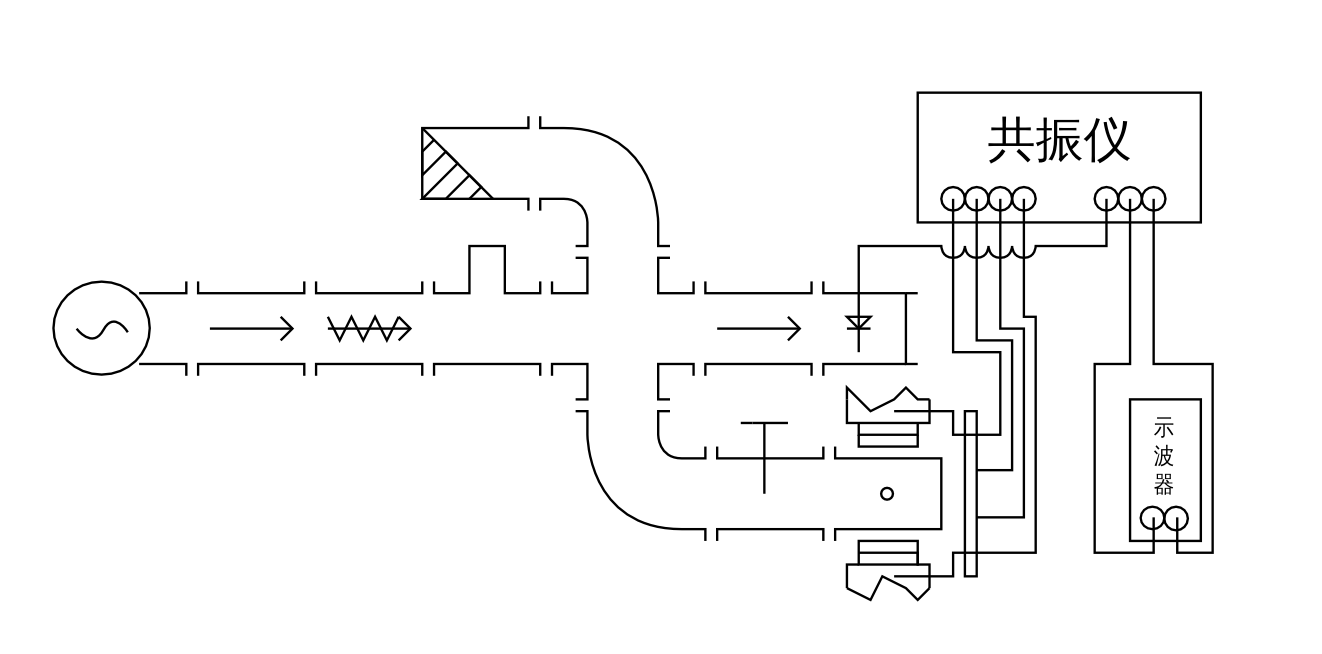
\includegraphics[width=0.8\textwidth]{pic1.png}
		\caption{\label{fig:exp1}马赫——曾得干涉仪示意图。激光器打出来的激光经过两面凸透镜扩束形成平行光,经过分束板形成两路相干的平行光束后重新汇聚相干于干板。}
	\end{center}
\end{figure}

激光扩束调整后形成的平行光束经过马赫——曾得干涉仪的调整,形成了两条相干的平行光。如果这两条光束严格的平行,则在屏幕的x方向上就不会形成干涉条纹。而如果两束平行光有一定的夹角,则在X方向上出现了干涉条纹,当角度越大的时候,干涉条纹越密集。

我们认为两束平行光与屏幕法线方向的夹角分别为$\theta_1$和$\theta_2$,且另$\omega=\theta_1+\theta_2$为两束光的会聚角。由杨氏干涉实验中的计算可以得到干涉条纹之间的间距为:
\begin{equation}
	d=\frac{1}{\nu}=\frac{\lambda}{\sin \theta_1+\sin \theta_2}=\frac{\lambda}{2\sin{(\frac{\theta_1+\theta_2}{2})}\cos{(\frac{\theta_1-\theta2}{2})}}
\end{equation}
式子中$\lambda$是激光束的波长,当$\theta_1=\theta_2$而且其和非常小的时候,近似有:\begin{equation}
	d\approx\frac{\lambda}{\omega}
\end{equation}
在本次实验中因为会聚焦并不大所以可以根据上式估测光栅空间频率。

从式子中可以看出,调整$\theta_1$和$\theta_2$的大小可以影响形成的正弦衍射图样的空间密度。对应一个频率曝光后,改变空间频率再曝光一次,即可吧频率为$\nu$和$\nu+\Delta\nu$的两个平行光栅拍摄在同一个干版上。这时候干版的总曝光量为:
\begin{equation}
	E=E_0+\cos{2\pi\nu\xi}+\cos{2\pi(\nu+\Delta\nu)\xi}
\end{equation}
式中$\xi$为空间坐标,正确的控制曝光显影条件,可以使得透射振幅与照到干版上的曝光量E成线性关系,则有光栅的投射率为:
\begin{equation}
	t=A-\beta[\cos{2\pi\nu\xi}+\cos{2\pi(\nu+\Delta\nu)\xi}]
\end{equation}
式中A是一个常数。这样制作出来的光栅即为复合光栅,当$\Delta\nu$不大的时候可以看到明暗相间的条纹被称作莫尔条纹,其空间频率为$\Delta \nu$。

\subsubsection{复合光栅的空间滤波}

\begin{figure}[h]
	\begin{center}
		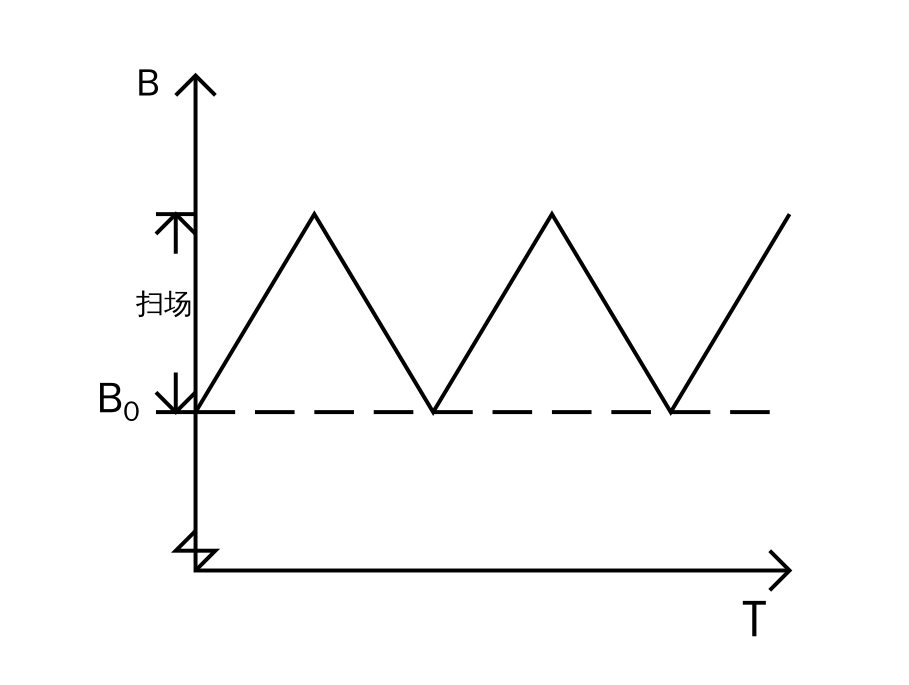
\includegraphics[width=0.8\textwidth]{pic2.png}
		\caption{\label{fig:exp2}相干光学处理系统(4F系统)示意图。L1,L2是两面傅氏透镜,P1,P2,P3都在透镜的焦点上。}
	\end{center}
\end{figure}

一束平行光照射物屏P1,经过透镜在L1的后焦面上得到频谱函数的傅立叶变换,在经过L2后边换回了原函数,只是变成了倒像。在频谱面P2处插入空间滤波器即可以改变频谱函数,从而使得输入的信号得到处理。

我们假设物屏面P1给出的复振幅分布为$g(x_0,y_0)$,则透镜L1会对其进行傅立叶变换,有
\begin{equation}
	\mathscr{F} \{ g(x_0,y_0) \} =G(f_\xi,g_\eta)
\end{equation}
其中$G(f_\xi,g_\eta)$是物函数的空间频谱,以
$$f_\xi=\frac{\xi}{\lambda F}\ \, f_\eta=\frac{\eta}{\lambda F}$$
所以其复振幅可以写作
\begin{equation}
	U_1(\xi,\eta)=G(\frac{\xi}{\lambda F},\frac{\eta}{\lambda f})
\end{equation}

经过复合光栅L2之后可以得到在P2面的复振幅为:
\begin{equation}
	U_2(\xi,\eta)=U_1(\xi,\eta)t(\xi)
\end{equation}
其中
$$t(\xi)=A-B\{\exp{(i2\pi\nu\xi)}+\exp{(-i2\pi\nu\xi)}+\exp{[i2\pi(\nu+\Delta\nu)\xi]}+\exp{[-i2\pi(\nu+\Delta\nu)\xi]}\}$$
为光栅的振幅透着率。

经过L2进行的傅立叶分解可以得到,其像的复振幅满足:
\begin{equation}
	\begin{split}
	U_(x,y)\propto Ag(x,y)-B\{g(x-\nu\lambda F,y)+g(x+\nu\lambda F,y)\}\\-B\{g[x-(\nu+\Delta\nu)\lambda F,y]+g[x+(\nu+\Delta\nu)\lambda F,y]\}
	\end{split}
\end{equation}

所以可以看出经过复合光栅相当于经过了两个正弦光栅。此时两个光栅处于相位相同,所以得到的一级衍射条纹相互加强。如果调整使得两个光栅的相位相反(即$\xi=0$处于莫尔条纹的暗处时候)有光栅波函数改变为:
 
$$t(\xi)=A-B\{\exp{(i2\pi\nu\xi)}+\exp{(-i2\pi\nu\xi)}-\exp{[i2\pi(\nu+\Delta\nu)\xi]}-\exp{[-i2\pi(\nu+\Delta\nu)\xi]}\}$$

最后的复振幅为
\begin{equation}
	\begin{split}
	U_(x,y)\propto Ag(x,y)-B\{g(x-\nu\lambda F,y)+g(x+\nu\lambda F,y)\}\\+B\{g[x-(\nu+\Delta\nu)\lambda F,y]+g[x+(\nu+\Delta\nu)\lambda F,y]\}
	\end{split}
\end{equation}

当$\Delta\nu$相对小的时候可以写成微分形式:
\begin{equation}
	U_3(x,y)\propto Ag(x,y)-B\left.\frac{\partial g}{\partial x}\right|_{x=-\nu\lambda F}\cdot\Delta\nu\lambda F+B\left.\frac{\partial g}{\partial x}\right|_{x=+\nu\lambda F}\cdot\Delta\nu\lambda 
\end{equation}

在这种情况下如果屏面图像是简单的矩形,则如下面的示意图所示轮廓会清晰的凸显出来。

\begin{figure}[h]
	\begin{center}
		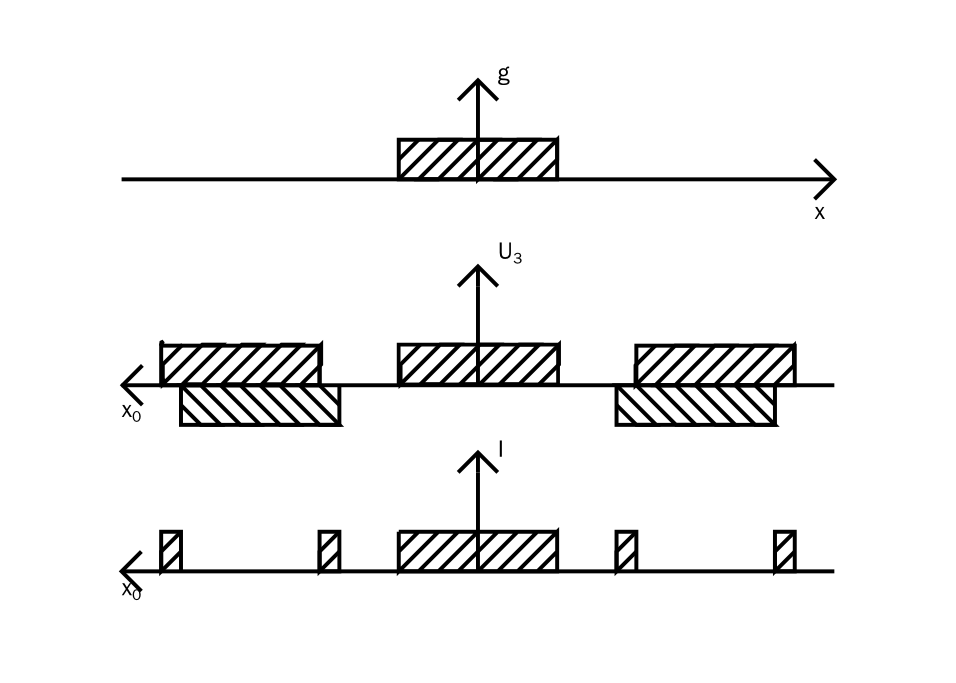
\includegraphics[width=0.8\textwidth]{pic3.png}
		\caption{\label{fig:exp3}(上图) P1平面输入信号,(中图) P3平面复振幅分布,(下图)P3平面光强分布。}
	\end{center}
\end{figure}

\subsection{实验步骤以及数据}

首先按照马赫——曾得干涉仪调整光路。将激光器打出来的激光束扩束调整平行,经过分束镜子形成两束相干光,然后汇聚到一起。这时候尽量调整两束品行光使其都与水平面平行。也就是最后的两束平行光经过一个透镜后在后焦面上形成的两个光点完全的重合,同时在调整汇聚光的分束镜子的时候,光点移动的方向应该与光学平台平面平行。

轻微调整汇聚两束平行光的分束境,这时候应该可以明显的在接收屏幕上看到明暗相间的相干竖直直条纹。这时候即可证明调整的没有问题。本实验制作的光栅的空间频率在70条每毫米左右,激光的波长为632.8nm,带入先前的公式可以得到,需要得到两束光的会聚角$\omega=\nu\lambda=4.43\times10^{-2}$。即在经过焦距为190mm的汇聚透镜后焦点上的两个光点的距离应该为8.41mm。

通过估测可以知道使得两个光点移动8.41mm需要旋转分束镜旋钮4.25周左右,本实验需要制作$\Delta\nu\approx2 mm^{-1}$左右的复合光栅,计算可以得到对应的会聚角的变化为$\Delta\omega=1.27\times10^{-3}$即旋转分束境旋钮45度左右。

调整相干条纹空间频率为70条每毫米左右,然后在接受屏幕上放上干版,曝光2秒钟。随后调整分束境旋钮,改变空间频率后再次曝光2秒钟,即可以得到复合光栅样品。在灯光下可以看出明显的莫尔条纹。

按照上文所示图搭建4F系统,光源为平行激光,将复合光栅样品放置在P2处,使之条纹方向沿竖直方向,此时就可以观察到衍射图样。此时水平移动复合光栅会发现一级衍射条纹有敏感变化,当一级条纹最暗的时候,也正是图像微分处理的时候,这时候可以明显的看到图像边缘轮廓。如下图所示:
\newpage
\begin{figure}[h]
	\begin{center}
		\subfigure{
			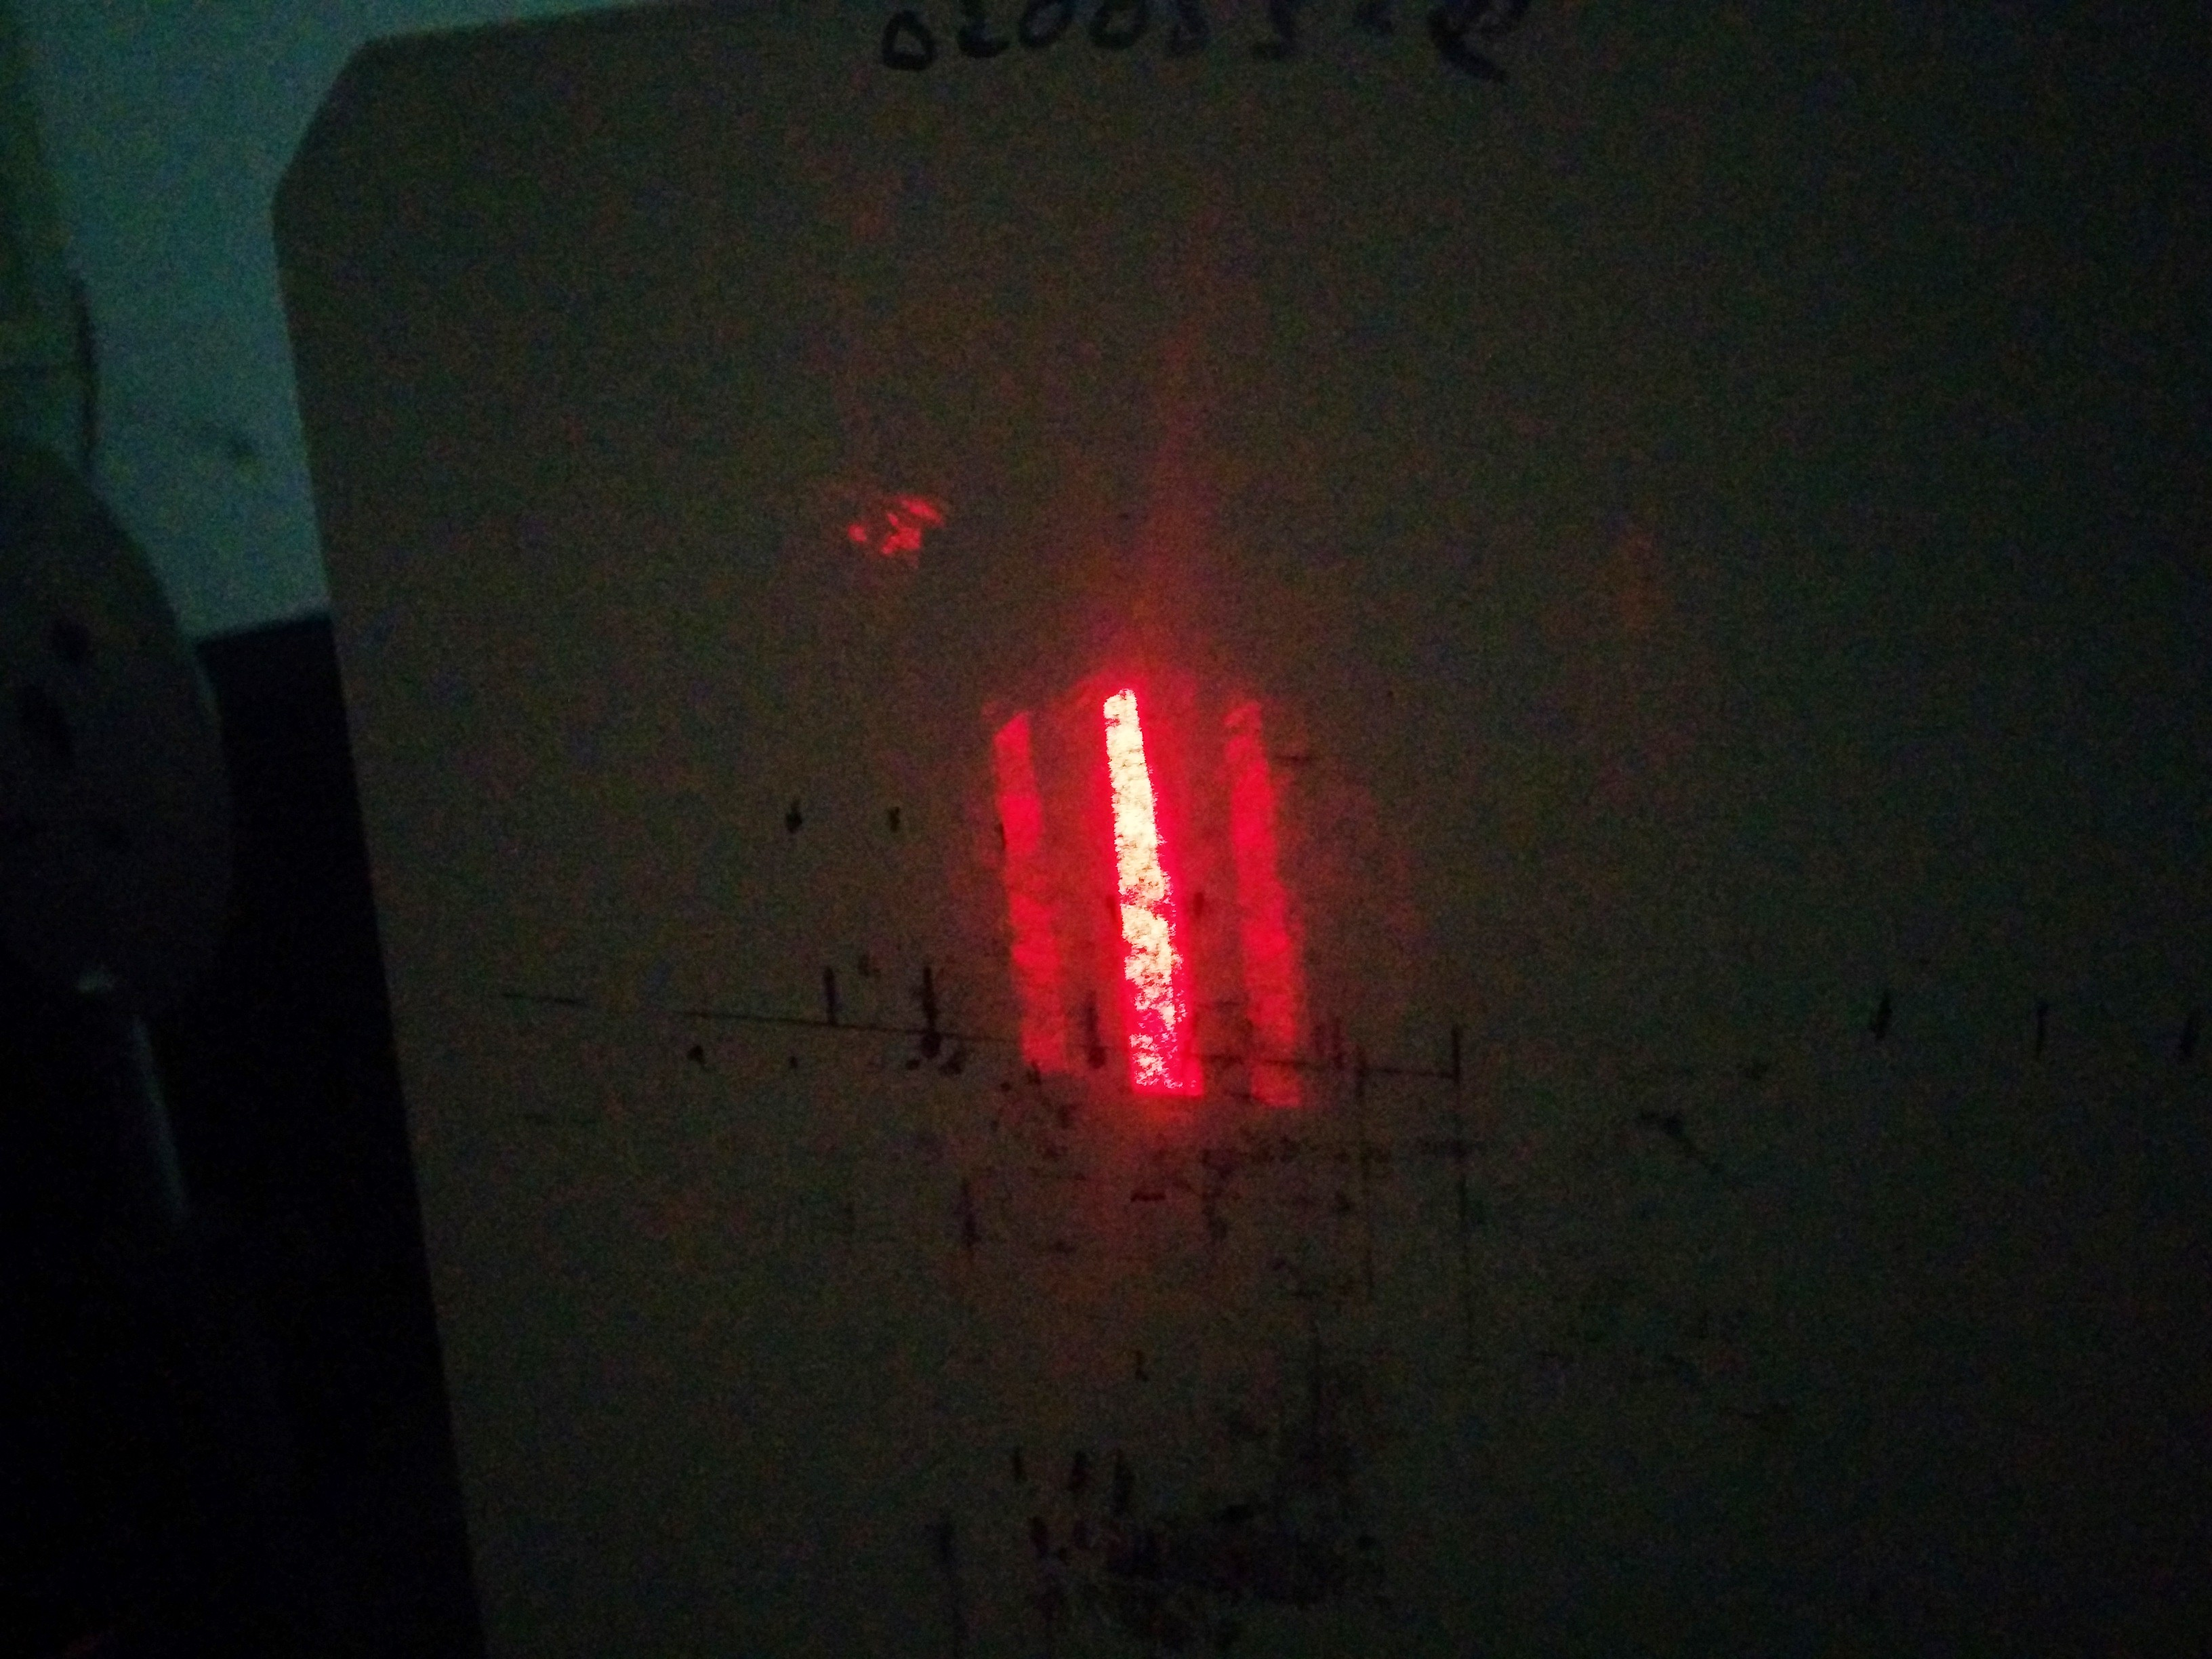
\includegraphics[width=0.4\textwidth]{pic4.jpg}}
		\subfigure{
			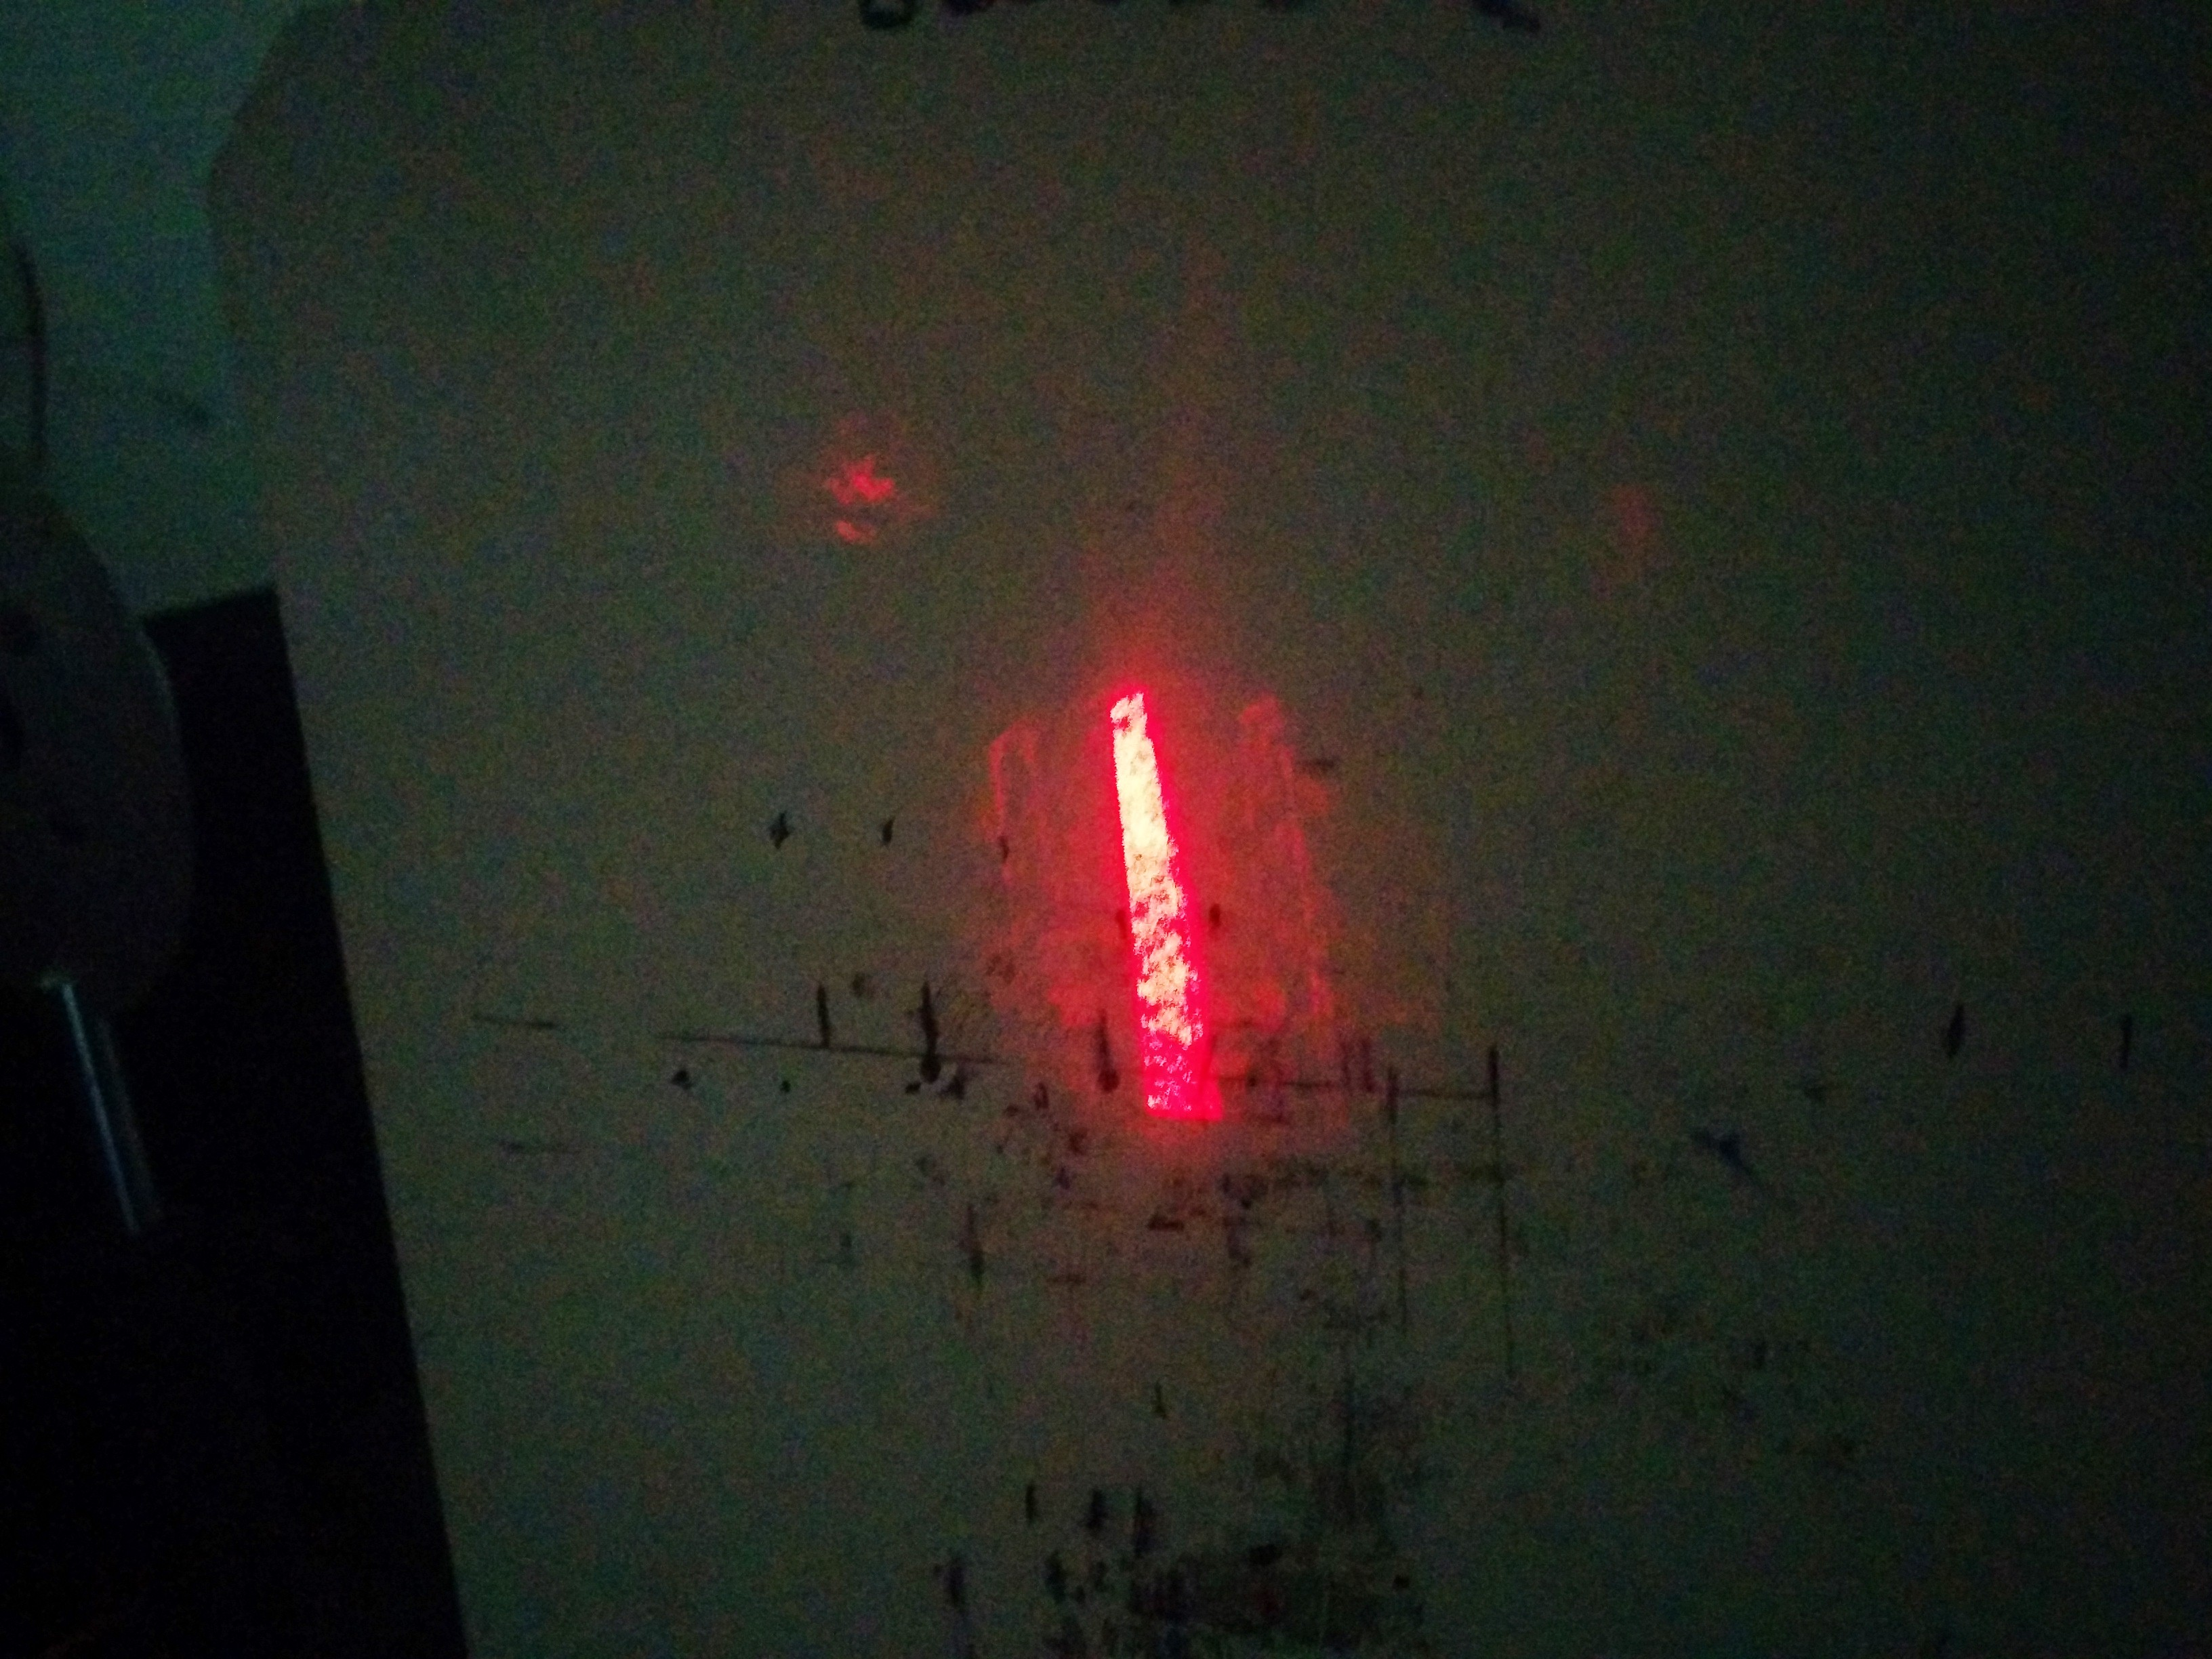
\includegraphics[width=0.4\textwidth]{pic5.jpg}}
		\caption{\label{fig:exp2}(左图)复振幅同相位光强叠加。(右图)复振幅相位相反图像微分。}
	\end{center}
\end{figure}

测量光栅周期频率,有测量得到一级衍射条纹距离主级条纹的间距为$\Delta x=0.89cm$。4F系统的焦距$l$为190mm。

接下来测量莫尔条纹的周期,水平移动复合光栅,同时测量一级衍射条纹极暗时的位置。数据如下:

\begin{center}
	\begin{table}[h]
		\caption{衍射条纹极暗时符合光栅的位置}
		\begin{tabularx}{15cm}{r|XXXXXXXXX}
			\hline
			微分图像位置&1&2&3&4&5&6&7&8&9\\
			\hline
			位置/mm&0.201&0.518&0.885&1.227&1.543&1.885&2.225&2.564&2.874\\
			\hline
		\end{tabularx}
	\end{table}
\end{center}


\section{数据分析及讨论}

带入公式计算可以得到光栅的周期频率有:
$$d=\frac{\lambda}{\sin{\theta}}\approx\frac{\lambda}{\theta}=\frac{dl}{\Delta x}=73.5 mm^{-1}$$

对于莫尔条纹进行拟合可以得到:

\begin{figure}[h]
	\begin{center}
		\includegraphics[width=0.8\textwidth]{pic6.eps}
		\caption{\label{fig:exp3}莫尔条纹间距拟合图像。图像表示再出现第i个微分图像时候符合光栅的水平位置}
	\end{center}
\end{figure}
\newpage
可以看出来其线性程度非常的高,计算可以得到空间频率$\nu=\frac{1}{b}=2.98 \pm 0.02 mm^{-1}$

对于图像微分的瑕疵,应该是由于光学器件并不是十分的干净,这个在移动复合光栅的时候可以明显的观测的像平面上有不规则的图样随之移动。同时因为光栅是振幅投射性质的光栅,其对于衍射条纹的衰减是十分明显的,也就显得一级衍射条纹十分的暗淡,不易观测到。再加上物并不是毛玻璃而是平行光经过光阑,光强十分的大,自身图样会因为衍射而形成光晕使得观察更不容易,综合起来导致了图像微分的效果不是十分的优良。

\section{结论}

这次实验利用马赫——曾得干涉仪制作出了复合光栅,并配合4F系统进行了光学图像的微分系统的实验,得到了预期的结果,验证了利用复合光栅可以实现光学图像微分的结论。并对制作出来的复合光栅进行了一定的测量。得到其周期间距为:
$$\nu=73.5mm^{-1}$$
以及摩尔条纹的周期为:
$$\Delta\nu=2.98 \pm 0.02 mm^{-1}$$。

 
\section{致谢}
感谢赵子强老师的指导,以及贾春燕,冉书能老师的技术支持。



\begin{thebibliography}{}
	\bibitem{Book} 吴思成,王祖铨~2010 近代物理实验(第三版)(北京:高等教育出版社)第371页.
	\bibitem{Book2} 宋菲君,陈树源~近代光学信息处理 (北京大学出版社) 
%
%
\end{thebibliography}

\clearpage
\appendix
\section{思考题}

\end{document} 
